\section{Aufbau und Durchführung}
\subsection{Aufbau}
Der Messaufbau besteht im Kern aus einem radioaktiven Isotop und einem
Geiger-Müller-Zählrohr, welches die auftretenden Zerfälle registriert (siehe Abbildung \ref{fig:aufbau}).
\begin{figure}[H]
\centering
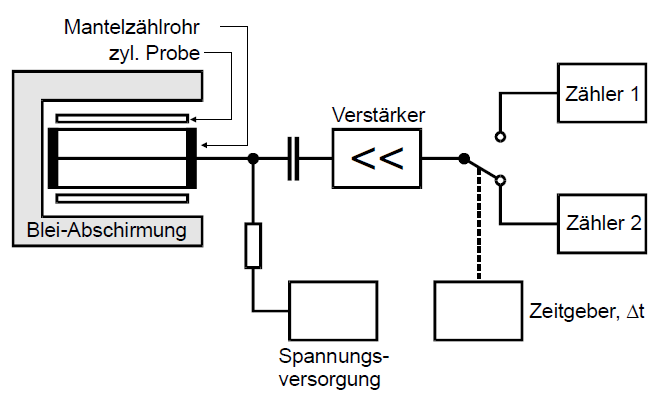
\includegraphics[width = 10cm, height= 7cm]{Schematisch.png}
\caption{Eine schematische Darstellung des Messaufbaus. \cite{1}}
\label{fig:aufbau}
\end{figure}
\noindent  
Dieses besteht aus einer mit Argon 
gefüllten Röhre. Trifft nun ein Betateilchen oder ein Gammaquant auf das Argon, wird dieses ionisiert und 
sorgt aufgrund einer hohen anliegenden Spannung für eine Elektronenlavine. Die Spannung kann anschließend 
ohne einen größeren Verstärker gemessen werden. Die Messzeit kann am Ausgabegerät des Zählrohrs eingestellt
werden. Nach einem Durchlauf wird auf ein zweites Zählwerk gewechselt, sodass die aktuellen Ergebnisse notiert werden können. 
Zusätzlich ist der Messaufbau mit einer Bleikleidung versehen. Zum einen schirmt Sie das Messgerät 
vor verfälschender kosmischer Strahlung ab, zum anderen schützt Sie den Anwender vor der vorherrschenden 
Radioaktivität. Um die benötigten radioaktiven Isotope zu erzeugen, werden stabile Kerne in einem Behälter
nach mit Neutronen beschossen. Um die Ausbeute zu maximieren durchlaufen die Neutronen 
zunächst jedoch eine bremsende Paraffinschicht.
\subsection{Duchführung}
Als erstes wird eine Messung für den Nulleffekt $N_U$ durchgeführt.
Um Fehler aufgrund von Störquellen, wie kosmischer Strahlung, zu minimieren wird zunächst ein Leerlauf 
ohne Isotop über $\text{600}\text{s}$ durchgeführt. 
Nun folgt zunächst eine Zerfallsmessung des Elementes Vanadium. Die Vanadium-Probe wird in das Geiger-Müller-Zählrohr gesteckt, 
wie in Abbildung \ref{fig:Aufbau1} dargestellt ist.
\begin{figure}[H]
    \centering
    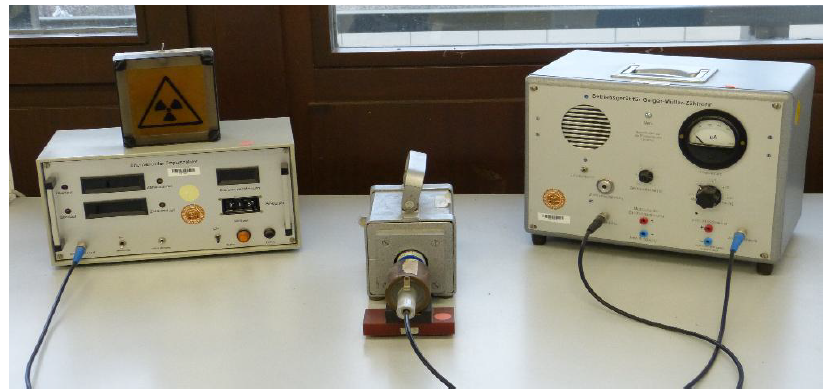
\includegraphics[width = 10cm, height= 7cm]{Aufbau.png}
    \caption{Der Versuchsaufbau. \cite{1}}
    \label{fig:Aufbau1}
\end{figure}
\noindent
Es wird in einem Intervall von $\Delta t$=30 s gemessen.
Anschließend wird die Vanadium-Probe durch den Rhodium-Probe ausgetauscht. Diesmal wird 
die Messung in einem Zeitintervall von $\Delta t$=15 s gemessen.

\label{sec:Aufbau und Durchführung}
